

% quantum impurity problem,  boundary critical phenomena, Anderson orthogonality catastrophe
In (one-dimensional) quantum critical systems, the presence of the physical boundary and isolated impurity weakly break the conformal symmetry. Simply put, the interface scatters the otherwise independent modes and therefore demonstrates novel boundary critical phenomena\cite{cardy_boundary_2004}. Operators close to the boundary are interpreted as boundary condition changing (bcc) operators\cite{oshikawa_boundary_1997,affleck_boundary_1997} in the boundary conformal field theory (CFT). Their correlation functions can exhibit different critical exponents from their bulk counterparts\cite{cardy_conformal_1984}. One example is the ``Anderson orthogonality catastrophe", where the core hole creates a potential that acts as an impurity to the conduction band. The X-ray absorption rate will then have a power law singularity of a boundary exponent\cite{affleck_boundary_1997} at the resonance frequency. There are numerous impurity problems of this kind that have been studied in the last few decades, such as the magnetic impurity in the spin chain\cite{eggert_magnetic_1992}, boundary and impurity effects in Luttinger liquid\cite{fabrizio_interacting_1995}, entanglement of the defects\cite{peschel_entanglement_2005, igloi_entanglement_2009,calabrese_entanglement_2012} \etc

% non-equilibrium dynamics, particle mediate the two parts, Cardy cut-and-join protocol, Vassur majarana
Recently, more attention has been paid to the non-equilibrium dynamics of quantum impurity\cite{hegde_quench_2015,francica_local_2016,lupo_transient_2016,lee_spatiotemporal_2016,chung_memory_2016,sacramento_edge_2016,vasseur_expansion_2015,mazza_overlap_2016}. The ``cut-and-join" quench protocol is a popular framework for investigating the spreading of the influence from the localized impurity (or boundary) across the system. As shown in the left panel of Fig.~\ref{fig:cut-and-join}, the system consists of two critical chains A and B, which were prepared in the ground states. They will be joined at $t = 0$ and evolve. Various quantities can be used to detect the information in the quench process. For instance, Ref.~\onlinecite{calabrese_entanglement_2007, calabrese_quantum_2016} find a logarithmic increase of entanglement entropy in subsystem A, when both A and B are identical critical systems. The authors ascribe such increase to the proliferation and propagation of the quasi-particle excitations emitted at the joint. Ref.~\onlinecite{vasseur_universal_2014} takes A to be a normal lead and B to be a topological superconductor in the topological phase. In this model, the Majorana zero mode acts as a bcc operator and its conformal dimension appears in the exponent of the power law decay of the Loschmidt echo.

\begin{figure}[h]
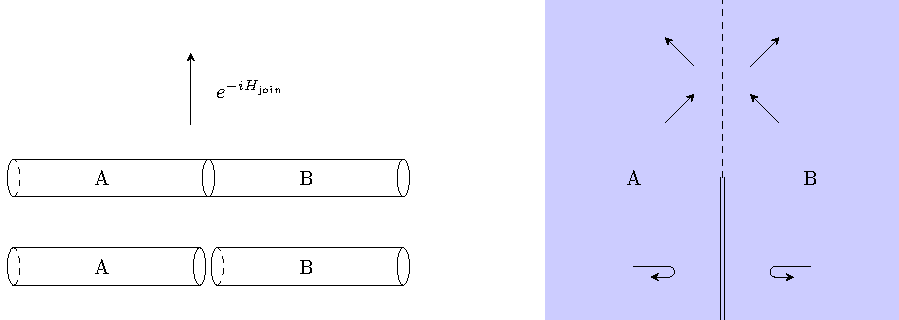
\includegraphics[width=1\columnwidth]{fig_cut_and_join.pdf}
\caption{Cut-and-join quench protocol. Left panel: Prepare the ground states of the two separated chains and join them at $t = 0$, then time evolve with the whole chain Hamiltonian. Right panel: Spacetime diagram of the cut and join protocol. The solid line represents the boundaries of the two disconnected chains. It is totally reflective for the incident particles on both sides. The dashed line is the world line of the junction, which we will call interface. It could either be totally transparent or partially permeable, depending the types of theories of A and B.}
\label{fig:cut-and-join}
\end{figure}

% All of these are the same CFTs. we consider different CFTs, the mediating particle or primary field will be different, from the S matrix point of view.
In the path integral language, the ``cut-and-join" protocol corresponds to a spacetime diagram as shown in the right panel of Fig.~\ref{fig:cut-and-join}. The separating ground states prepared before $t = 0$ are joined to form a new type of interface between them. Before the quench, the slit represents boundaries that are completely reflective to the injecting particles. During the quench, the joining turns on the transmission from one side to the other. In the entanglement entropy and Loschmidt echo examples cited above\cite{calabrese_entanglement_2007, calabrese_quantum_2016, vasseur_universal_2014}, the two sides of the CFTs are the same (chiral fermion CFT in the case of Ref.~\onlinecite{vasseur_universal_2014}) and the boundary becomes totally transparent after the joining. 

In this paper, we generalize these ideas to an interface that interpolates between the totally reflective and complete transparent ones. This kind of interface can have many realizations. As discussed in Ref.~\onlinecite{bachas_permeable_2002}, one can connect two different bosonic CFTs in the ``cut-and-join" protocol, and the interface is a domain wall between two free compact boson theories with different compactification radii. Such permeable interface can also be implemented by non-compact free boson/fermion on a lattice with a fine-tuned bond interaction between the boundary sites (see \onlinecite{peschel_exact_2012,sakai_entanglement_2008} for their entanglement property studies). In these models, there is a parameter $\lambda$ that is directly related to the transmission coefficient. In the case of the compact boson, $\lambda$ is controlled by the ratio of the compactification radii, while for the free lattice boson it is controlled by the ratio of masses. We expect it to be tunable in a realistic experimental setting.

% fidelity and Loschmidt echo are quantities that extract boundary critical exponents, may reveal the nature of the mediating particle 
We compute the Loschmidt echo to extract information in the dynamics of the quench process of these models. The Loschmidt echo is the (square of the) overlap of the wavefunctions before the quench and the wavefunction evolved for some time $t$. It decays with a power law $t^{- \alpha}$ for the lack of length scale in the $t \rightarrow \infty$ limit. The decay exponent $\alpha$ has been calculated for various geometries and combinations of normal boundary conditions of the same CFTs in \onlinecite{stephan_logarithmic_2013,stephan_local_2011}. We extend the analysis to the aforementioned parametric interface of (possibly) different CFTs. We will see that there are two categories of the scattering matrices $S(\theta)$ of the interfaces, whose scattering angle parameter $\theta$ is determined by the transmission coefficients. Our analytic and numerical results show that $\alpha$ has a quadratic dependence on the change of $\theta$ if the prior and post quench boundary conditions are in the same type of $S$, while remaining $\frac{1}{4}$ otherwise. The finite size fidelity calculation further supports these results. 

The rest of the paper is organized as follows. In Sec.~\ref{sec:bosonic_conformal_interface}, we introduce the general formalism for the permeable bosonic conformal interface and its lattice realization. In Sec.~\ref{sec:analytic_numerics}, we analytically evaluate the free energy associated with the fidelity and Loschmidt echo, and present the numerical results for comparison. We discuss our results and related experimental works in Sec.~\ref{sec:disc}. Finally, we conclude in Sec.~\ref{sec:conclusion}. 

This paper includes several appendices for technical details. In App.~\ref{app:lambda_12}, we present the leading order analytical calculation of the free energy for the setups in Sec.~\ref{sec_sub:analy_eval}. In App.~\ref{app:gnd_dn_lambda}, we illustrate an alternative approach with one setup as an example. In App.~\ref{app:F_correction}, we point out two corrections to the free energy, which are complementary to the argument made in the main text. Up to this point, we work exclusively with the oscillator modes of the free bosons. In App.~\ref{app:compact_diff_boson}, it is shown that the winding modes of the compactified bosons will \emph{not} contribute to the free energy at the leading order. Therefore, the results remain valid in the physical situation of connecting two compactified bosons of different radii. In App.~\ref{app:pf_of_id}, we prove one identity that will be used repeatedly in the analytical evaluation. We derive the scale invariant interface for the free bosonic lattice in App.~\ref{app:interface_free_boson}. The details of the numerical simulation are presented in App.~\ref{app:comp_fid_echo}.

%%% Local Variables:
%%% TeX-master: "bCFT_paper"
%%% TeX-PDF-mode: t
%%% End:
